\documentclass[11pt,final]{scrbook}
\usepackage[paper=a4paper, twoside, bindingoffset=5mm, headheight=20pt, top=20mm, bottom=40mm,left=25mm,right=35mm]{geometry}
\usepackage[utf8]{inputenc} 	% UTF-8 (Unicode) encoding
%\usepackage{fullpage}
\usepackage{boxedminipage}
\usepackage{varioref}
\usepackage{amsmath,amssymb}    % Mehr Mathe Befehle (z.B. \text{})
\usepackage{minitoc}
\usepackage{graphicx}           % Grafiken einfach einbinden
\usepackage{epstopdf}
%\usepackage[export]{adjustbox}
\usepackage{scrpage2}           % Für Kopfzeilen
\usepackage{tabularx}           % tollere Tabellen
\usepackage{multirow}
\usepackage{booktabs}
\usepackage{array}
\usepackage{units}
\usepackage[squaren, thinspace]{SIunits}
\usepackage{soul} % letter s p a c i n g

% Andere Schriftart als Standard:
% Palatino for rm and math | Helvetica for ss | Courier for tt
\usepackage{mathpazo} % math & rm
\linespread{1.05}        % Palatino needs more leading (space between lines)
\usepackage[scaled]{helvet} % ss
\usepackage{courier} % tt
\normalfont
\usepackage[T1]{fontenc}
\usepackage{subfigure}          % mehrere Graphen in einem
\usepackage{caption}
\usepackage{paralist}

\def\Nabla{\bm{\nabla}}
\def\bm{\mathbf}
\def\curl{\Nabla\times}
\def\div{\Nabla\cdot}
\def\lap{\Delta}
\def\vlap{\Delta}
\def\x{\hat{e}_{x}}
\def\y{\hat{e}_{y}}
\def\z{\hat{e}_{z}}
\def\p{\partial}
\def\h{\hat}
\def\tw{\tilde{\omega}}
\def\gm{\gamma}
\def\om{\omega}
\def\OM{\Omega}
\def\GM{\Gamma}
\def\dw{\delta\omega}
\def\dth{\Delta\theta}
\def\dk{\delta k}
\def\Hdth{\frac{\dth}{2}} %half Delta Theta
\DeclareMathOperator{\Tr}{Tr}

% Alter some LaTeX defaults for better treatment of figures:
% See p.105 of "TeX Unbound" for suggested values.
% See pp. 199-200 of Lamport's "LaTeX" book for details.
%   General parameters, for ALL pages:
\renewcommand{\topfraction}{0.9}	% max fraction of floats at top
\renewcommand{\bottomfraction}{0.8}	% max fraction of floats at bottom
%   Parameters for TEXT pages (not float pages):
\setcounter{topnumber}{2}
\setcounter{bottomnumber}{2}
\setcounter{totalnumber}{4}     % 2 may work better
\setcounter{dbltopnumber}{2}    % for 2-column pages
\renewcommand{\dbltopfraction}{0.9}	% fit big float above 2-col. text
\renewcommand{\textfraction}{0.07}	% allow minimal text w. figs
%   Parameters for FLOAT pages (not text pages):
\renewcommand{\floatpagefraction}{0.7}	% require fuller float pages
% N.B.: floatpagefraction MUST be less than topfraction !!
\renewcommand{\dblfloatpagefraction}{0.7}	% require fuller float pages

%Farbe
\usepackage{color}
\definecolor{gray}{gray}{0.95}

% Zeilenabstand
\usepackage{setspace}
%\linespread{1.5}
\onehalfspacing

% Code samples
\usepackage{listings}
\lstset{numbers=left, numberstyle=\tiny, numbersep=5pt, stepnumber=1}
\lstset{language=}
\lstset{frame=leftline}
\lstset{basicstyle=\footnotesize\ttfamily, stringstyle=\ttfamily}
\lstset{moredelim=[is][\bfseries]{|*}{*|}}
\lstset{backgroundcolor=\color{gray}}


% Hyperref
\usepackage[square,comma,numbers]{natbib}
\usepackage[pagebackref, pdfborder={0 0 0}]{hyperref}
\renewcommand*{\backref}[1]{}% for backref < 1.33 necessary
\renewcommand*{\backrefalt}[4]{%
	\ifcase #1 % 
		\textit{No citations.}%
	\or
		\textit{Cited on page #2.}%
	\else 
		\textit{Cited on pages #2.}%
	\fi
}%

% last \usepackage
% ============================
% 

% Programmierung von Armin Dobner für Bildunterschriften (slanted)
 \makeatletter
 \renewcommand{\fnum@figure}{{\bfseries \figurename~\thefigure}}
 \renewcommand{\fnum@table}{{\bfseries \tablename~\thetable}}
 \long\def\@makecaption#1#2{%
   \vskip\abovecaptionskip
   \sbox\@tempboxa{#1{\bfseries :} {\slshape #2}}%
   \ifdim \wd\@tempboxa >\hsize
     #1{\bfseries :} {\slshape #2}\par
   \else
     \global \@minipagefalse
     \hb@xt@\hsize{\hfil\box\@tempboxa\hfil}%
   \fi
   \vskip\belowcaptionskip}
 \makeatother



% Absätze
\setlength{\parskip}{1.5ex plus0.3ex minus0.3ex}
\setlength{\parindent}{0pt}

\clubpenalty = 10000
\widowpenalty = 10000

% Kommandos
\newcommand{\code}[1]{{\tt #1}}
\newcommand{\class}[1]{\code{\textbf{#1}}}
\newcommand{\keyword}[1]{\class{#1}}
%\newcommand{\sf}[1]{\textsf{#1}}
%\newcommand{\eqref}[1]{equation~(\ref{#1})}

\renewcommand\ohm{\text{$\Omega$}}
\newcommand{\siox}{SiO$_\text{2}$}

%Konstanten
\newcommand{\Boltz}{k_{\text{B}}}
\newcommand{\psibi}{\psi_{bi}}
\newcommand{\pH}{\text{$p$H}}


% trennung
\hyphenation{dia-me-ter}
\hyphenation{na-no-tu-be}
\hyphenation{na-no-scale}

%Kopfzeile
\pagestyle{scrheadings}
\automark[section]{chapter}
\setlength{\headheight}{3\baselineskip}
\setheadsepline{0.5pt} % Linie oben Zeichnen
\ihead{} %links oben
\chead{}
\lehead{\thepage  \hspace{4em} Chapter \headmark} % rechts oben
\rohead{\headmark \hspace{4em} \thepage}
\ofoot[]{} % Seitenzahl in der Fußzeile entfernen

%\titlehead{\textbf{Technische Universität München \\ Institut für Nanoelektronik \hfill 2011}}
%\title{Carbon Nanotube Thin Film Devices for Biological Sensors}
%\author{Tobias Haeberle}
%\date{\today}

\dedication{To my friends and family.}


% ============================
%  DOCUMENT START
% ============================
\begin{document}

%%
%% Titel-tex
%%
%
%% Die vertikalen Abstände nach Eingabe der Daten bitte selbst anpassen.
  % title page

\begin{titlepage}
%\raggedleft\includegraphics{figures/Universitaet_Logo_RGB.pdf}
\begin{center}
    
\includegraphics[width=\textwidth]{images/Logos2.pdf}% [scale=0.7, right]
    
    \vspace{25mm}	
    
    {
        \scshape	
        Technische Universität München\\
        Fakultät für Elektrotechnik und Informationstechnik\\																										% 
        Professur für Computational Photonics\\
        Prof.Dr.-Ing. Christian Jirauschek
    }
		
    \vspace{25mm}																								

    \begin{LARGE}
        \normalfont\rmfamily \textbf{Coupled Transmission Line/Maxwell-Bloch Equations Approach for Electro-Optical Simulations of Terahertz Quantum Cascade Lasers}\\[6cm]
    \end{LARGE}
   \so{\Large MASTER THESIS}\\[0.5cm]
    
    by Longwei Zhong

    \textbf{May, 2017}\\[2cm]
																	
 																	
\end{center}

\end{titlepage}

\clearpage \thispagestyle{empty} \cleardoublepage 




\pagenumbering{roman}



\chapter*{Abstract}
\addcontentsline{toc}{chapter}{Abstract}
Quantum cascade lasers (QCLs) are compact, electrically pumped semiconductor devices, which are considered to be promising light source for mid-infrared and terahertz radiation. Benefit from this special mechanism they can utilize the electric power more efficiently than other diode lasers and achieve a high output power. Despite its practical significance, generating ultra short pulses from QCLs by mode-locking has achieved only limited success in the past decade. In this work, we study the influence of external source on the mode-locking of QCLs. A dynamic model based on Maxwell-Bloch equations as well as transmission line was build to simulate QCLs in time domain. The simulation results were then analyzed and compared with existing experiment results from references to check reliability of the established model.

The purpose of this research is to build a new model based on existed simulation methods to achieve a dynamic modeling of QCLs in time domain, which would help to get a better understanding of its theoretical mechanism and redound to still unresolved issues of the field.

\chapter*{Acknowledgements} 
\addcontentsline{toc}{chapter}{Acknowledgements}

Thanks to Petar

\clearpage
\thispagestyle{empty}

\vspace*{2cm}
\begin{center}
{\normalfont\itshape  I dedicate this work to my beloved mother and father}
\end{center}

\chapter*{List of Symbols}


% ============================
%  Content
% ============================

\tableofcontents

\chapter{Introduction}\pagenumbering{arabic}
The operating principle of QCLs was first proposed by R.F. Kazarinov and R.A. Suris in 1971 \cite{kazarinov1971possibility}. However, due to the complexity of fabrication process until 1994 QCLs was firstly demonstrated at Bell Laboratories by Jerome Faist and his colleagues\cite{faist1994quantum}. They have gained considerable attention afterwards. Unlike common semiconductor lasers, which utilize electron-hole recombination to realize electromagnetic radiation, QCLs are unipolar and their emission is based on intersub- band transitions in coupled quantum well superlattices\cite{williams2007terahertz}. Due to lack of suitable radiation sources and detectors this region remains one of the least developed spectral regions. The occurance of QCLs provides a option as a prominent source to help investigate these regions, because their emission wave length as well gain spectrum can be engineered through various design \cite{gmachl2002ultra}. 

To date, only n-type QCLs are successfully realized lasing, the intersubband transmission occurs in conduction band. 

Introduction of materials used for QCL

\section{Background and motivation}
There are already several successful experimental attempts by active mode locking so far, but a complete theory system is still not available due to limited knowledge of quite complex mechanism inside cavity, both electrical as well as optical. It has been proven to be difficult to directly employ existing techniques from the ultra fast optics community to mode-lock QCLs due to unfavorable physical effects and lack of consolidation theory about its mechanism. Despite various obstacles some clear mode-locking of QCLs has been realized already in the mid-infrared as well as terahertz. All of the attempts are based on active mode-locking, which was recognized as the only viable route to QCL mode locking \cite{revin2016active}. The main idea is to actively mode-lock the QCLs through a modulated injection current with a frequency corresponding to the round-trip frequency $f_{rt}$, which lies in the microwave region extending from around 3 kHz to 300 GHz.

The first successful attempt in mid-IR QCLs was achieved in 2009 \cite{wang2009mode} by modulating a short section of the cavity to open a net gain window. Different with common QCL design (Bound to continuum, Chirped superlattice, Resonant-phonon, Hybrid/interlaced), the QCL that was used is based on a "diagonal transition", which was a specially designed and owns significant longer gain recovery time. It was found that mode-locked pulses can be formed by modulating current injection close to the laser threshold, while high above threshold pulses are broadened due to multi-mode instabilities (Spatial Hole Burning and RNGH-instability).

Recently active mode locking of QCLs in an external ring cavity was reported \cite{revin2016active}, which can operate at room temperature. Moreover, benefits from this method, the mode-locking was observed not only at close to the threshold, but also far above it. 

Similar to mode-locking in mid-IR, THz QCLs can also be injection locked by active mode-locking with an external RF source. Besides, it was found that mode-locking in THz QCLs is easier than that in mid-IR. Compared with mid-IR QCLs, the laser transition energy lies below the optical phonon energy, so the upper state of THz QCLs based on bound-to-continuum has generally longer non-radiative relaxation time ($\sim$ 5-10 ps), which makes it easier to mode-lock \cite{barbieri2011coherent}. The first successful attempt of mode-locking in THz QCLs was reported in 2010 \cite{gellie2010injection}. The same with in mid-IR QCLs, they also used RF modulation to achieve mode-locking with a modulation frequency corresponding to the round trip frequency of the laser. By direct amplitude modulation, the mode-locking of a 2.3THz QCL was achieved at 35GHz with input RF-power <-15dBm.

In the last two decades many studies have been carried out on further development as well as possible applications of QCLs. Some groups devoted themselves to improve the operation temperature, up to room temperature has been achieved\cite{bai2011room} through special wells design of QCL structure. Some consisted on generating short pulse by using QCLs\cite{wang2009mode}. Besides, In the past few years researchers have showed high interest in the application of QCLs. There are already many 
....


\section{Related work}
Accompanied with investigation of QCLs in experiments, theoretical modeling techniques are developed step by step.

\section{Objective}
The objectives of this thesis are as follows:

1). To build a new dynamic model 

2). To verify "pulling effect" in mode-locking through simulation

3). To acquire optimal simulation parameters to generate short pulse

4). To gain a deep understanding of mode-locking behaviors to obtain a better design in the future.

\chapter{Theory}
\section{Maxwell-Bloch equation}
\section{Transmission line}
Transmission line model was created by Oliver Heaviside \cite{heaviside2008electromagnetic} and usually consists of two separated conductors and medium in between (Fig. \ref{fig:TLcircuit}). The conventional TLM is based on Telegrapher's equations (\ref{eq:TLequation1})(\ref{eq:TLequation2}), which describe the evolution of voltage and current both spacial and temporal on an electrical transmission line. These two differential equations contains four distributed components (R', L', G', C') which vary from different transmission lines: R' is distributed resistance of conductors, which is represented by a series resistor in ohms per unit length ($\Omega /m$); L' is distributed inductance resulting from the magnetic field around the line due to self-inductance, which is represented by a series inductor in henries per unit length ($H/m$); G' is distributed conductance of the dielectric material separating the two conductors, which is expressed in siemens per unit length ($S/m$) and represented by a shunt resistor with resistance of 1/G'; C' is distributed capacitance of transmission line, which is represented by a shunt conductor in farads per unit length ($F/m$).

Transmission line can be further classified in lossy/non-lossy transmission line and uniform/nonuniform transmission line with regarding to characteristics of its conductors and medium. When no resistance (idea conductor) and conductance (idea dielectric medium) exist, it can be regarded as ideal transmission line which contains only L' and G'. In uniform transmission line all those distributed components are uniformly distributed along line. Therefore, under the assumptions above the simulated QCL can be defined as a 1D nonlinear lossy transmission line.\\

% TL equivalent circuit figure
\begin{figure}[htbp]
\begin{center}
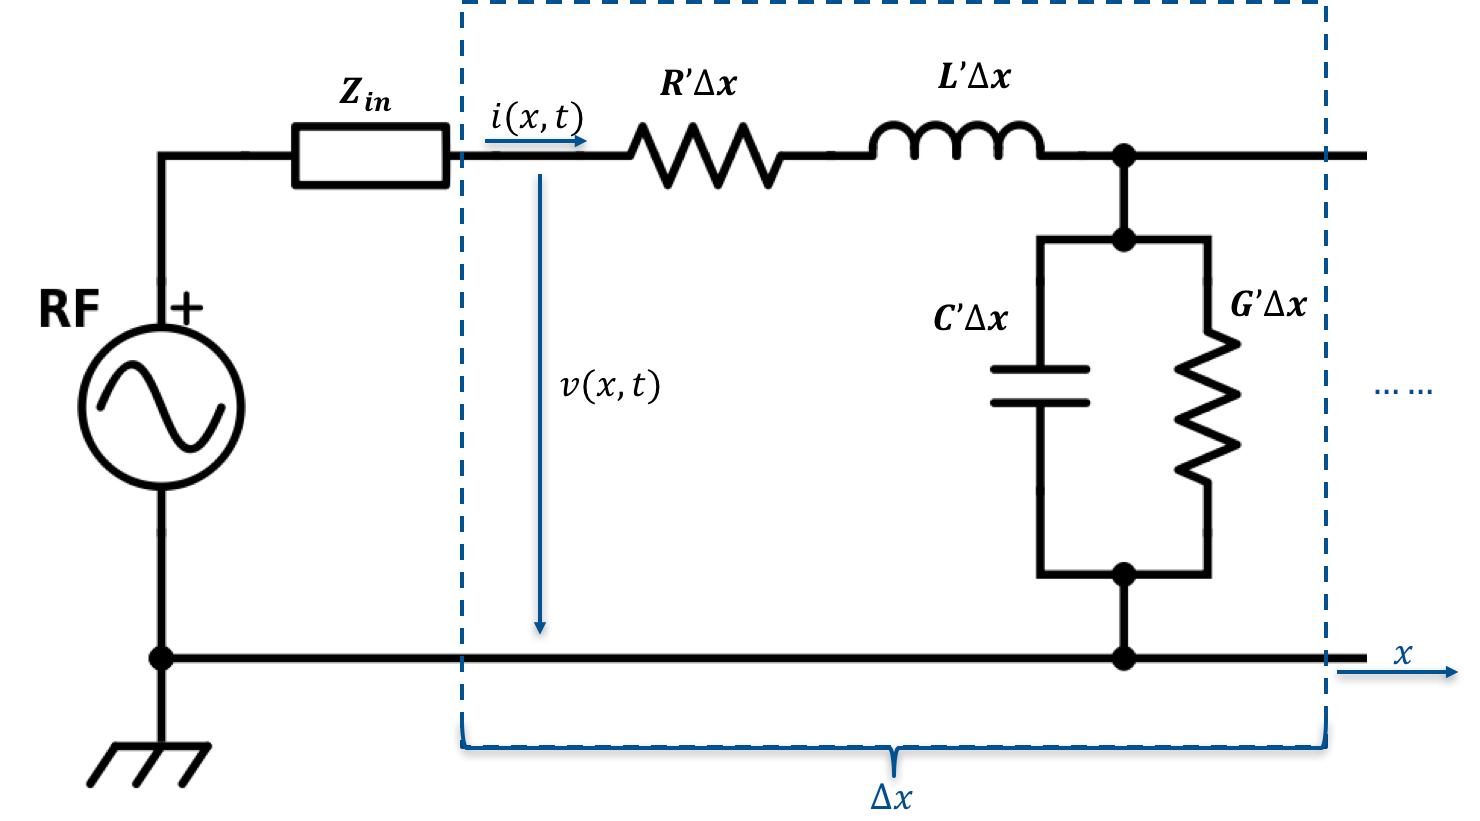
\includegraphics[scale=0.4]{images/TLcircuit}
\caption{: An equivalent circuit representation of a differential section of the waveguide with capacitance per unit length C’ and inductance per unit length L’.}
\label{fig:TLcircuit}
\end{center}
\end{figure}
% Transmission line equations
Telegrapher's equations:
\begin{eqnarray}
\frac { \partial v(x,t) }{ \partial x }  &=& -L'\frac { \partial i(x,t) }{ \partial t }-R'i(x,t) \label{eq:TLequation1}\\
\frac { \partial i(x,t) }{ \partial x }  &=& - C'\frac { \partial v(x,t) }{ \partial t }-G'v(x,t) \label{eq:TLequation2}
\end{eqnarray}

\section{Mode-locking}
Mode-locking is a technique in optics, which locks multi-mode in resonant laser cavity by enforcing coherence between modes to produce extra short pulse\cite{haus2000mode}. Methods of mode-locking can be simply classified in active mode-locking (AML) and passive mode-locking(PML) depending on whether it is modulated by itself (e.g. absorber) or requires external modulation source (e.g. RF source).

fundamentals of mode-locking knowledge.....
\chapter{Model}
\section{Optical modeling}
Similar with the existing modeling methods, in this model light propagation is described with Maxwell' equation while carrier transportation is determined by Bloch equation. Without regard to lateral non-uniform distribution at boundaries \cite{huang2014non, dhar2015nanoscopic} QCL can be simplified to one-dimensional (1D) structure in the direction of propagation (x axis), which means the electrical components were uniformly distributed throughout the cross-sectional area. 

\subsection{Carrier transport}
****-->rewrite, give more details about density matrix model

To simulate QCL active regions, we adapt the density matrix model from Ref. [cite Belyanin], to include total of four subband levels, and more importantly to allow all relevant system parameters, such as the eigenenergies, dipole moments and all scattering rates to be bias dependent. 

As a prototypical QCL design, we take the sub-band structure configuration illustrated in Fig. \ref{fig:4Levels}, consisting of 4 relevant levels per period, i.e. levels from 1 to 4, where level 4 denotes the upper laser state, level 3 the lower laser level, level 2 is an extraction level which eases the electron extraction from 3, and finally level 1 denotes the depopulation level of the period, which also coincides with the injector state (1') of the next module. Typical QCL designs consist of more than 30 repetitions of this schematic, however we can employ periodic boundary conditions [cite] and restrict our attention to a single period only. 

\begin{figure}[htbp]
\begin{center}
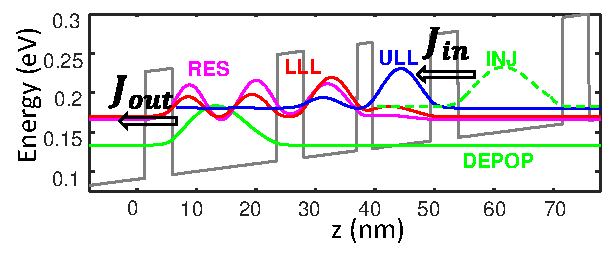
\includegraphics[scale=1.2]{images/WFs.pdf}
\caption{Sub-band structure configuration of QCL.}
\label{fig:4Levels}
\end{center}
\end{figure}

The time evolution of the density matrix is given by the von Neumann equation, which we couple to a wave equation for $E_z(x,t)$, denoting the $z$-component electric field (and also the assumed laser growth direction).  
\begin{subequations}
	\label{eq:dmequations}
 \begin{align}
	\frac{d\rho_{44}}{dt} &= J +i\frac{ez_{43}}{\hbar}E_z(\rho_{43}-\rho_{34}) + \sum_{j\neq 4} \frac{\rho_{jj}}{\tau_{j\rightarrow 4}}  - \frac{\rho_{44}}{\tau_{4}}, \\
	\frac{d\rho_{33}}{dt} &= -i\frac{ez_{43}}{\hbar}E_z(\rho_{43}-\rho_{34}) + \sum_{j\neq 3} \frac{\rho_{jj}}{\tau_{j\rightarrow 3}} - \frac{\rho_{33}}{\tau_{3}}, \\
	\frac{d\rho_{22}}{dt} &= \sum_{j\neq 2} \frac{\rho_{jj}}{\tau_{j\rightarrow 2}} - \frac{\rho_{22}}{\tau_{2}}, \\
	\frac{d\rho_{11}}{dt} &=  -J + \sum_{j\neq 1} \frac{\rho_{jj}}{\tau_{j\rightarrow 1}} - \frac{\rho_{11}}{\tau_{1}}, \\
	\frac{d\rho_{43}}{dt} &= - i\omega_{43}\rho_{43} + i\frac{ez_{43}}{\hbar}E_z(\rho_{44}-\rho_{33})-\Gamma_{\parallel 43}\rho_{43}.
 \end{align}
\end{subequations}
In Eqs. (\ref{eq:dmequations}) $\rho_{ij}$ denotes the $ij-$th density matrix element,  $z_{43}$ the optical transition's dipole moment, $e$ the elementary charge, $\hbar$ is the reduced Plank's constant. Also the parameter $1/\tau_{i\rightarrow j}$ is the net scattering rate from level $i$ to level $j$, calculated by our ensemble Monte Carlo code and incorporating, amongst others, longitudinal optical (LO) phonon, interface roughness and electron electron scattering mechanisms [cite]. Lastly $1/\tau_{i} = \sum_j 1/\tau_{i\rightarrow j}$ is the inverse lifetime of level $i$ and $\Gamma_{\parallel 43} = (\tau_4+\tau_3)/(2\tau_4\tau_3)+1/\tau^*$ is the dephasing rate of the optical transition, including lifetime broadening and a phenomenological pure dephasing $1/\tau^*$ rate due to intrasubband scattering processes [cite ANDO model]. The only scattering mechanism treated quantum mechanically is the optical transition between the upper and lower laser states. One can also fully coherently include resonant tunneling between the injector 1' and the upper laser state 4, which leads to a modified system of equations with larger number of independent variables and is thus more computationally demanding [cite]. Furthermore such an approach does not allow for the inclusion (without $k-$space discretization) of second order tunneling current into the simulations, which has been shown to be the origin of negative the differential conductivity and dispersive gain  in quantum cascade lasers []. This is why in this publication we adhere to the more intuitive model from [cite Belyanin], which can be easily adapted to include various models for the current density via the term $J$ in the above equations. Keeping in foresight that we would like to couple the density matrix equations to an electrical model for the waveguide, we find the later model as the more suitable alternative.

In the tight-binding basis [cite], we can assume that the only electron transport channel across the QCL periods is via the resonant tunneling current between the injector and the upper laser state. When second order scattering effects are considered, under a few relaxing approximations, this tunneling current is given by [cite Terrazzi]
\begin{align}
\label{eq:current}
J &= en^s\frac{\Omega_{AC}^22\Gamma_{\parallel 1'4}}{\epsilon^2+4\Gamma_{\parallel 1'4}^2}\Big\{\Theta(\epsilon)(\rho_{11}-\rho_{44}e^{-|\hbar\epsilon|/k_BT}) \nonumber \\
&+\Theta(-\epsilon)(\rho_{11}e^{-|\hbar\epsilon|/k_BT}-\rho_{44})\Big\}.
\end{align}
In Eq. (\ref{eq:current}) $n^s$ denotes the sheet carrier density, $\Theta(\cdot)$ is the Heaviside function and the term $e^{-|\hbar\epsilon|/k_BT}$ denotes an effective "weight" factor modelling the assumption of thermalized $k$-space distribution of the injector and upper laser level electrons with the same thermal energy $k_BT$ in each subband.   

\subsection{Light propagation}
****-->rewrite, give more explanation for concept polarization P

In order to include the electric field dynamics into the overall picture, we write down the inhomogeneous wave equation 
\begin{align}
\label{eq:waveqn}
\left [\frac{c^2}{n_{THz}^2} \frac{\p^2}{\p x^2} -\frac{\p^2}{\p t^2} \right ] E_z =\frac{1}{\epsilon_0 n_{THz}^2}\frac{\p^2}{\p t^2}P,
\end{align}
where  $n_{THz}$ denotes the background refractive index of the bulk active region, $c$ is the velocity of light in vacuum and $\epsilon_0$ is the permittivity of free space. The symbol $P$ denotes the (nonlinear) polarization of the two level system and is given by 
\begin{equation}
P(x,t) =  -\frac{n^s}{L_p}\Gamma ez_{43} (\rho_{43}+\rho_{34}),  
\end{equation}
with $\Gamma$ is the field confinement factor and $L_p$ is the period length. 

For the final set of equations, we also employ the rotating wave and slowly varying envelope approximations [cite], which allows us to reduce  the wave equation (\ref{eq:waveqn}) to a pair of propagation equations, an also eliminate fast oscillating terms from the density matrix equations (\ref{eq:dmequations}). The corresponding final formulas are slightly modified versions of those in [cite me, cite belyanin], and therefore we omit them here for brevity. We would like to point out also that in all subsequent calculations, we have also taken into consideration the effect of the inversion grating on to the current density, in an analogous manner to [cite belyanin]. 

\section{Electrical modeling}
In the electrical modeling, a modified Transmission Line Method (TLM) was introduced in order to realize a dynamic modeling in time domain. TLM is a very efficient methode which is already widely used for evaluation and dynamic modeling especially in high frequency region where wave nature muss be taken into accout, for example, contact resistance extraction in organic field- effect transistors \cite{xu2010modified}, dynamic modeling of flow in pipelines \cite{johnston2014enhanced} etc. However, in QCLs are transverse magnetic (TM) modes \cite{yan2009directional} while TLM is specially for analysis of transverse electromagnetic (TEM) modes, in which neither electric nor magnetic field in the direction of propagation. The common used metal-metal waveguide (microstrip structure) in QCLs can be regarded as quasi-TEM structure, as the substrate ($ \sim $ 10 um) is quite thin in terms of wavelength (30 mm $ \sim $ 300 mm), and the width of strip conductor is very narrow ($ \sim $ 50 um) in terms of wavelength as well, therefore, a static analysis should be still perfectly adequate in this case.

\begin{figure}[htbp]
\begin{center}
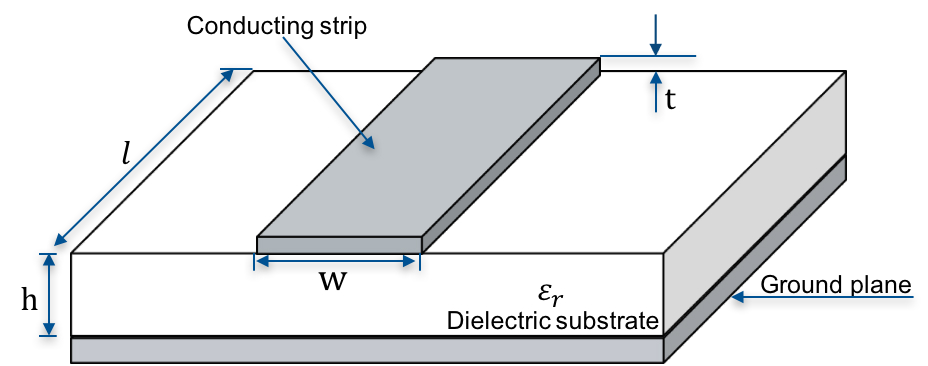
\includegraphics[scale=0.8]{images/Microstrip.pdf}
\caption{Microstrip structure.}
\label{fig:Microstrip}
\end{center}
\end{figure}

\subsection{Transmission line approach}
In this model, the vertical current component resulting from conductance of active region (n-doped semiconductor) under bias is calculated by current density J'(x,t) rather than by distributed conductance G'. Current density J(x,t) is nonuniform and bias dependent, it will be obtained by carrier transmission in optical part. 

\begin{eqnarray}
\frac { \partial v(x,t) }{ \partial x }  &=& -L'\frac { \partial i(x,t) }{ \partial t }-R'i(x,t) \label{eq:TLequation3}\\
\frac { \partial i(x,t) }{ \partial x }  &=& - C'\frac { \partial v(x,t) }{ \partial t }-wJ'(x,t) \label{eq:TLequation4}
\end{eqnarray}

\subsubsection{Boundary conditions}
Boundary conditions account for the completeness of differential equations at the boundary. In order to refine the boudaries and avoid hard variation of electrical components, a cascading of $\pi$ networks\cite{orlandi1996fdtd} is introduced for the distributed transmission line by splitting the shunt capacitance and conductance in half with two parallel capacitors and conductors at boundary, which is illustrate in Fig. \ref{fig:BoundaryCondition}. 

In active mode-locking, QCL is supplied with source $ {V}_{S} $ which consists of a DC voltage source $ {V}_{DC} $ and an external RF source $ {V}_{RF} $. These two sources are combined through bias-T and the source voltaged can be expressed with $ {V}_{S}=V_{DC}+{V}_{RF} $. As the right side of QCL lefts open, no current component exists at the end node. Consequently, the boundary condition for current is definitely ${I}_{end}^{n} = 0$. Besides, due to existance of wire impedance (50 $\Omega$) there will be voltage drop on it, so the voltage at node 0 is not equal to source voltage $ {V}_{S} $.
% Boundary condition figure
\begin{figure}[htbp]
\begin{center}
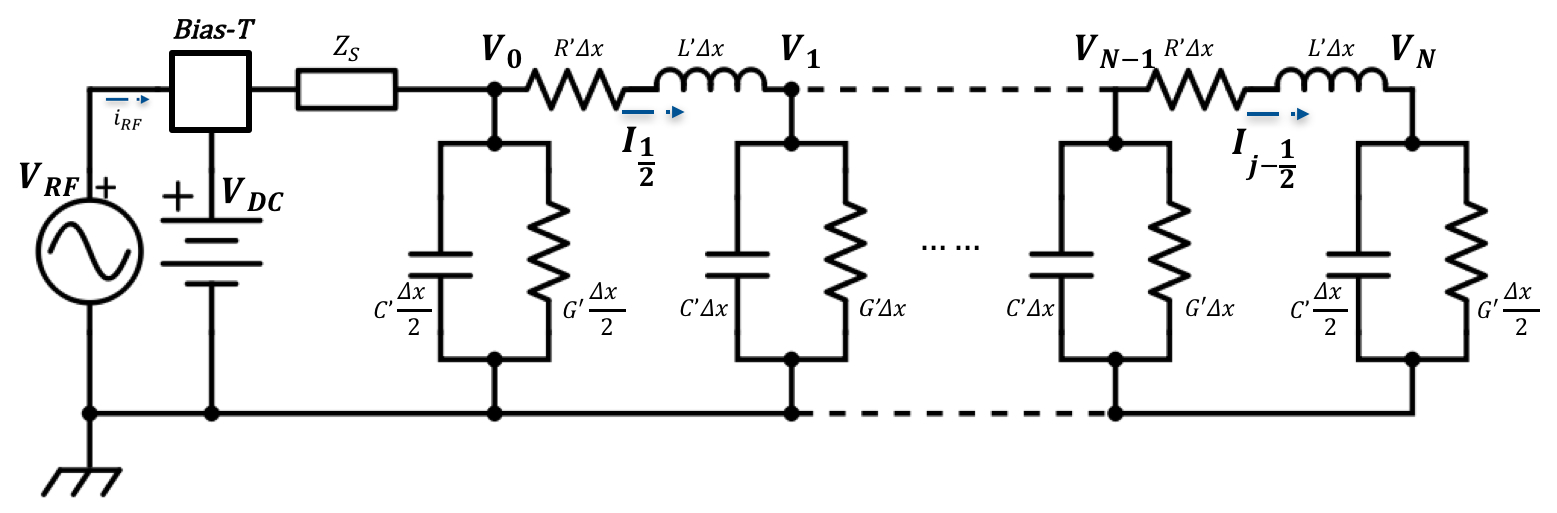
\includegraphics[scale=0.55]{images/pi_representation}
\caption{Schematic of cascade $\pi$ network representation and Thévenin equivalent circuit.}
\label{fig:BoundaryCondition}
\end{center}
\end{figure}

By using Kirchhoff's voltage law (KVL), 
\begin{equation}
{ V }_{ RF }^{n}+{V}_{DC} = {Z}_{S}\widetilde{ i }_{ -\frac{1}{2} }^{ n } + {V}_{0}^{n} \label{eq:Vs_n}
\end{equation}
where $\widetilde{ i }_{ -\frac{1}{2} }^{ n }$ denotes ac component among whole current after bias-T and before node 0. The same as in transmission line equation, it can not be directly calculated during iterative process. So by applying the same approximation treatment $\tilde{ i }_{ -\frac { 1 }{ 2 }  }^{ n+1 }-\tilde{ i }_{ -\frac { 1 }{ 2 }  }^{ n }\approx{ I }_{ -\frac { 1 }{ 2 }  }^{ n+1 }-{ I }_{ -\frac { 1 }{ 2 }  }^{ n }$, Eqn. (\ref{eq:Vs_n}) will be transformed to:
\begin{equation}
{ V }_{ RF }^{ n+1 }-V_{ RF }^{ n }={ V }_{ 0 }^{ n+1 }-V_{ 0 }^{ n }+Z_{ S }( { I } _{ -\frac { 1 }{ 2 }  }^{n+1}- { I } _{ -\frac { 1 }{ 2 }  }^{ n }) \label{Eq:boundary_V0}
\end{equation}

The injected current to QCL can be calculated through Kirchhoff's current law (KCL), at node 0:
\begin{align}
{ I }_{ -\frac { 1 }{ 2 }  }^{ n+1 }-{ I }_{ -\frac { 1 }{ 2 }  }^{ n }={ I }_{ \frac { 1 }{ 2 }  }^{ n+1 }-{ I }_{ \frac { 1 }{ 2 }  }^{ n }+C'\frac { \Delta x }{ 2 } (\frac { \partial V_{ 0 }^{ n+1 } }{ \partial t } -\frac { \partial V_{ 0 }^{ n } }{ \partial t } )+w\frac { \Delta x }{ 2 } (J_{ 0 }^{ n+1 }-J_{ 0 }^{ n })\label{Eq:boundary_ac}
\end{align}
Substitute Eqn. \ref{Eq:boundary_ac} into Eqn. \ref{Eq:boundary_V0}, and then rearrange the equation to get an explicit update expression at boundary:
\begin{equation}
{ V }_{ 0 }^{ n+\frac{3}{2} }=\frac{2Z_{S}C'\Delta x}{Z_{S}C'\Delta x+\Delta t}{ V }_{ 0 }^{ n+\frac{1}{2} }+\frac{ \Delta t-Z_{S}C'\Delta x }{Z_{S}C'\Delta x+\Delta t}{ V }_{ 0 }^{ n-\frac{1}{2} }+\frac{2\Delta t}{Z_{S}C'\Delta x+\Delta t}\big [{ V }_{ RF }^{ n+1 }-V_{ RF }^{ n }...
\end{equation}
\hspace{7cm}$- Z_{S}\big ({ I }_{ \frac { 1 }{ 2 }  }^{ n+1 }-{ I }_{ \frac { 1 }{ 2 }  }^{ n }+w\frac { \Delta x }{ 4 }(J_{0}^{n+\frac{3}{2}}-J_{0}^{n-\frac{1}{2}})\big )\big ]$


OR:$********************************************$

Use 40 GHz low loss RF coaxial cable which has 50 Ohms impedance.

$Z_{S}=\sqrt{\frac{L}{C}}=50\Omega$ (C = 27 pF/ft, L = 6.75e4 pH/ft, one foot length, 1 foot = 0.3048 m)

By using Kirchhoff's law, 
\begin{eqnarray}
{ V }_{ S }^{n+\frac{1}{2}}-{V}_{0}^{n+\frac{1}{2}} = L\frac{d{I}_{S}^{n+\frac{1}{2}}}{d{t}}\\\label{eq:BC_1}
{ I }_{ S }^{n+\frac{1}{2}} = { I }_{ \frac{1}{2}}^{n+\frac{1}{2}}+C\frac{d{V}_{0}^{n+\frac{1}{2}}}{d{t}}\label{eq:BC_2}
\end{eqnarray}
where ${ I }_{ S}$ denotes whole current from source after bias-T, which is relevant to current transmission from both RF and DC source. However, that cannot be directly obtained through iterative process. Substitute Eqn. \ref{eq:BC_2} to \ref{eq:BC_1}, leading to:
\begin{eqnarray}
{ V }_{ S }^{n+\frac{1}{2}}-{V}_{0}^{n+\frac{1}{2}} &=& L\frac{d{I}_{\frac{1}{2}}^{n+\frac{1}{2}}}{d{t}}+LC\frac{d^{2}{V}_{0}^{n+\frac{1}{2}}}{ dt^{2}}\\
&=& L\frac{{I}_{\frac{1}{2}}^{n+1}-{I}_{\frac{1}{2}}^{n}}{\Delta t}+LC\frac{{V}_{0}^{n+\frac{3}{2}}-2{V}_{0}^{n+\frac{1}{2}}+{V}_{0}^{n-\frac{1}{2}}}{(\Delta t)^{2}}
\end{eqnarray}
Then the equation above is rearranged to get an explicit update expression at boundary:
\begin{equation}
{ V }_{ 0 }^{ n+\frac{3}{2} } = (2-\frac{(\Delta t)^{2}}{LC}){ V }_{ 0 }^{ n+\frac{1}{2} }-{ V }_{ 0 }^{ n-\frac{1}{2} }+\frac{(\Delta t)^{2}}{LC}[V_{S}^{n+\frac{1}{2}}-\frac{L}{\Delta t}({I}_{\frac{1}{2}}^{n+1}-{I}_{\frac{1}{2}}^{n})]
\end{equation}


\subsubsection{Initial conditions}
Adequate initial conditions play a important role as well to acquire an accurate solution. However, real initial conditions for electrical distribution are not possible to be determined and verified. They can be only analytically set, which means a reasonable station at very beginning. In this case, supposing that QCL was biased by DC source barely at t$\leqslant 0$, no RF signal has arrived and no lasing yet. The following initial conditions are defined:
\begin{eqnarray}
V_{1}^{0} &=& V_{2}^{0} =...=V_{j}^{0}...=V_{N}^{0} = V_{DC}\\
I_{j+\frac{1}{2}}^{0} &=& I_{S}^{0}\times \frac{N-j}{N} \hspace{3mm} (j=0,1,2...,N-1)
\end{eqnarray}
where, $I_{S}$ is the initial current injection, which can be obtained by integrating J(x,0) over x from optical model. N is the amount of nodes while j integer ranging from 0 to N-1. The initial condition for current is under assumption that at very beginning the current was linearly distributed along active region in x direction.

\subsection{Distributed components}
The involvement of transmission line requires distributed component parameters. Except for distributed conductance G', which will be calculated in optical part, distributed resistance R', distributed inductance L' as well as distributed capacitance C' still need to be determined. They can be either calcuted as convertial passive components (plane resistor, parallel plane capacitor and inductor), or extracted from S-Parameter, which can be directly measured with network analyser. The former methode is simple and also don't require any extra test, but could lead to large error due to neglection of fringe effect\cite{pillai1970fringing} as well as high frequency influence. The latter is based on experiment, so shows higher accuracy compared with former, but requires extra experiment as well as equipment, which is not always feasible for simulation research. 

Distributed resistance is frequency dependent and can be obtained by measurement of S-parameter \cite{maineult2010microwave}, which shows constant value when under certain frequency $ R'=4.5\times10^{-5}\sqrt{f_{RF}}$ /mm.

\begin{equation}
R=\frac{1}{2(w+t)}\sqrt{\frac{\pi \mu f_{RF} }{\sigma}}
\end{equation}
where, $t$ is the thickness of top conductor, $\mu$ and $\sigma$ is the magnetic permeability coefficient and conductivity, respectively.

-->search corresponding parameters for gold at 77 K.....

\subsubsection{Distributed capacitance}
The cavity of QC laser is regarded as microstrip line in this case. Quasi-TEM structures, like microstrip, will have frequency dependent impedance and effective dielectric constant. However, if the substrate ($\sim$ 10 um) is thin in terms of wavelength (30 mm $\sim$ 300 mm), and if the strip conductor is very narrow ($\sim$ 50 um) in terms of wavelength, then a static analysis should be perfectly adequate.)

Numerically, one only have to consider a small, bounded 2D region with assumption of uniform cross-section going into the page (See Figure \ref{fig:Gauss2D}). 

\begin{figure}[htbp]
\begin{center}
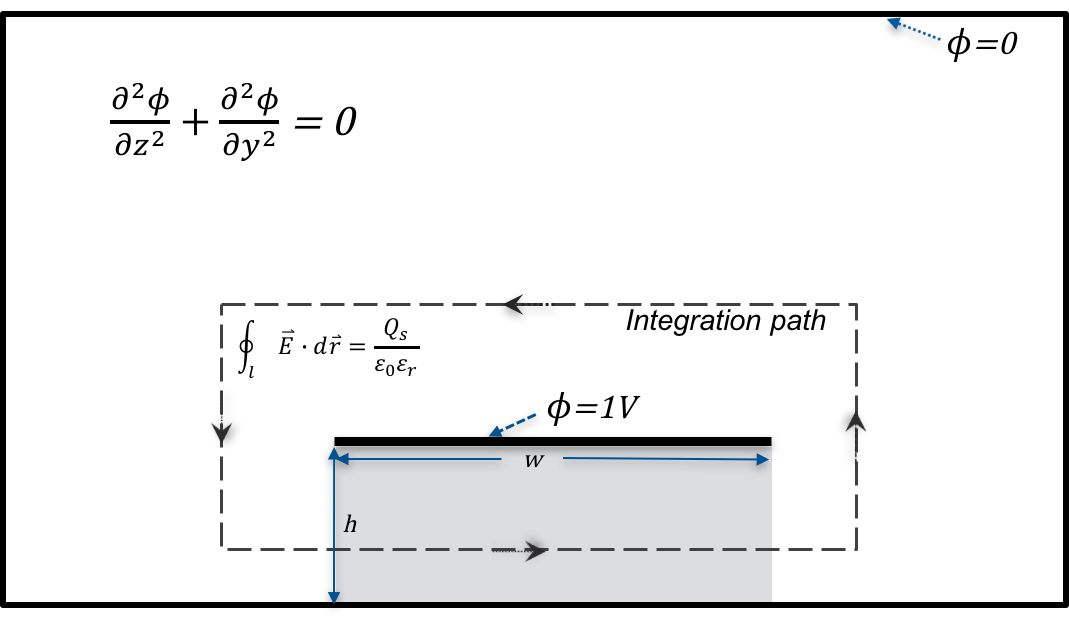
\includegraphics[scale=0.5]{images/Gauss2D.pdf}
\caption{Gauss's 2D equation.}
\label{fig:Gauss2D}
\end{center}
\end{figure}

The electric field can be solved by Gauss’s law in 2D. Solving for a strip in a box (Figure 2) the strip potential was set to 1V, the boundary to 0V and solve for the potential at a number of points inside the box. Here an electromagnetic field-solver QuickField was used which is a stand-alone software for solving partial differential equation (PDE). Figure 3 shows the calculated electric field around the strip.

\begin{align}
\frac { { \partial  }^{ 2 }\phi  }{ \partial { y }^{ 2 } } =\frac { { \phi  }_{ i-1,j }-2{ \phi  }_{ i,j }+{ \phi  }_{ i+1,j } }{ { (\Delta y) }^{ 2 } }\\
\frac { { \partial  }^{ 2 }\phi  }{ \partial { z }^{ 2 } } =\frac { { \phi  }_{ i,j-1 }-2{ \phi  }_{ i,j }+{ \phi  }_{ i,j+1 } }{ { (\Delta z) }^{ 2 } }
\end{align}

Set $\Delta y=\Delta z=\Delta$, then spacial electrical potential at each grid except top metal layer inside box can be resolved $ { \phi  }_{ i,j }=\frac { { \phi  }_{ i-1,j }+{ \phi  }_{ i+1,j }+{ \phi  }_{ i,j-1 }+{ \phi  }_{ i,j+1 } }{ 4\Delta ^{ 2 } } $


\begin{figure}[htbp]
\begin{center}
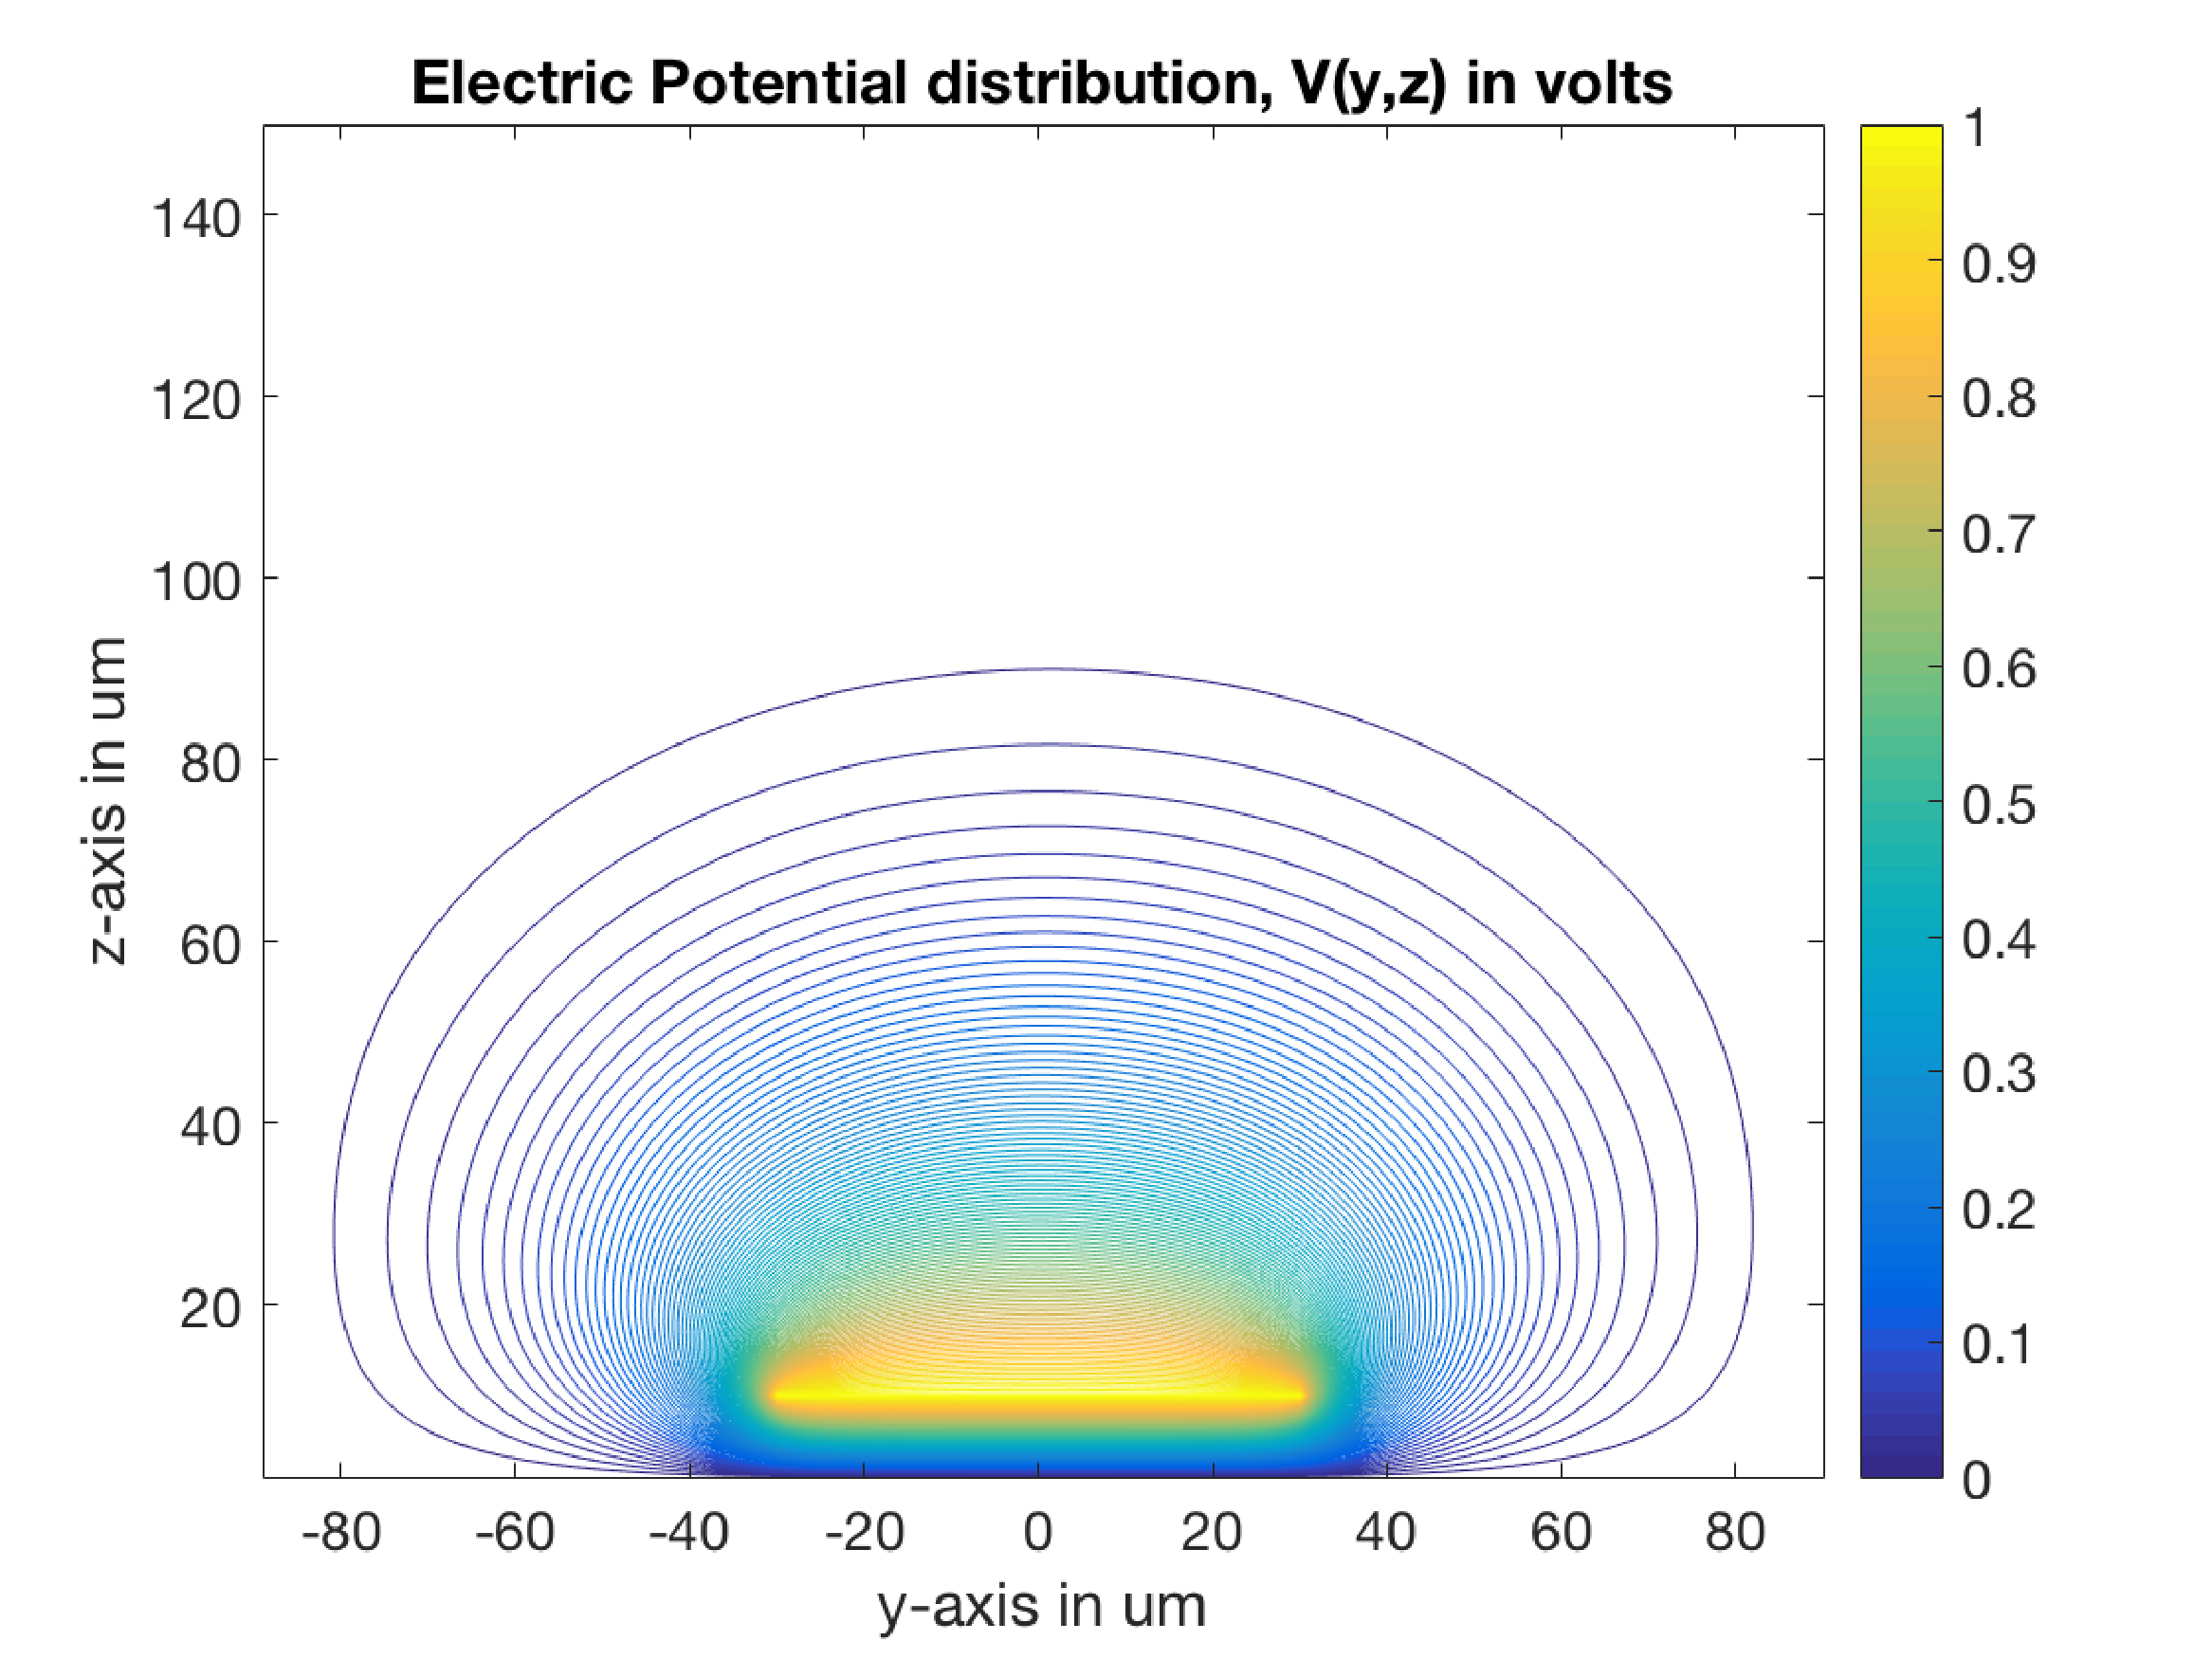
\includegraphics[scale=0.3]{images/TL_C.pdf}
\caption{Calculated electrical potential distribution V(y,z) with Matlab.}
\label{fig:TL_C}
\end{center}
\end{figure}

$E=-\nabla \phi$

pictures and calculations...

${ Q }_{ S }=\oint _{ l }{\varepsilon_{0}\varepsilon_{r}\overrightarrow { E } \cdot d\overrightarrow { r } } $
\subsubsection{Distributed inductance}
In order to evaluate the self-inductance of surface metal layer in QCLs, Biot–Savart law \cite{grant2013electromagnetism} is used for computing resultant magnetic field $\textbf{B}$ (SI unit: Tesla) at surrounding which is generated by a steady current $\textbf{I}$. The distributed inductance L is inhere characteristic for a certain metal or wire, and is independent of applied current value.  
\begin{equation}
\textbf{B}=\frac{\mu_{0}}{4\pi}\int _{ C }{ \frac { Id\textbf{l}\times \textbf{r} }{ |\textbf{r}| ^{3}}}
\end{equation}
where $\textbf{l}$ is the current unit length and $\textbf{r}$ is the displacement vector from current unit to the computed point, C is the path that current flows. Boldface denotes that symbols are vector quantities.

In QCLs with metal-metal structure, the thickness of top metal is usually extremely thin which is around 80 nm ($8\times 10^{-8} m$). Therefore, it can be regarded as a current sheet with assumption of no thickness (See Fig. \ref{fig:TL_L(2)}). The magnetic field resulting from a current unit is $d\textbf{B}_{P}=\frac { \mu \textbf{I}\times { \textbf{r}}dS }{ 4\pi w{ r }^{ 3 }}$ while the magnetic field at a point $ \textbf{B}_{P}$ results from the magnetic field of each current unit. Hence, it can be evaluated by adding all these together with superposition principle:
\begin{eqnarray}
 \textbf{B}_{P} &=& \sum _{ i=1 }^{ n }{ \sum _{ j=1 }^{ n }{ \frac { \mu \textbf{I}\times { \textbf{r} }_{ i,j } \Delta S }{ 4\pi w{ r }_{ i,j }^{ 3 } }  }  } \\
 &=& \int _{ -\frac { w }{ 2 }  }^{ \frac { w }{ 2 }  }{ \int _{ -\frac { l }{ 2 }  }^{ \frac { l }{ 2 }  }{ { \frac { \mu { \textbf{I} }\times { { \textbf{r} } }_{ i,j } }{ 4\pi w{ r }_{ i,j }^{ 3 } }  } }  } dxdy \label{eq. TL_L}
 \end{eqnarray}
 where, w is width of lateral cross section and $\textbf{r}$ is vector pointing from the surface element to the observation point P, $\mu$ is permeability depending on given medium and frequency.

 \begin{figure}[htbp]
\begin{center}
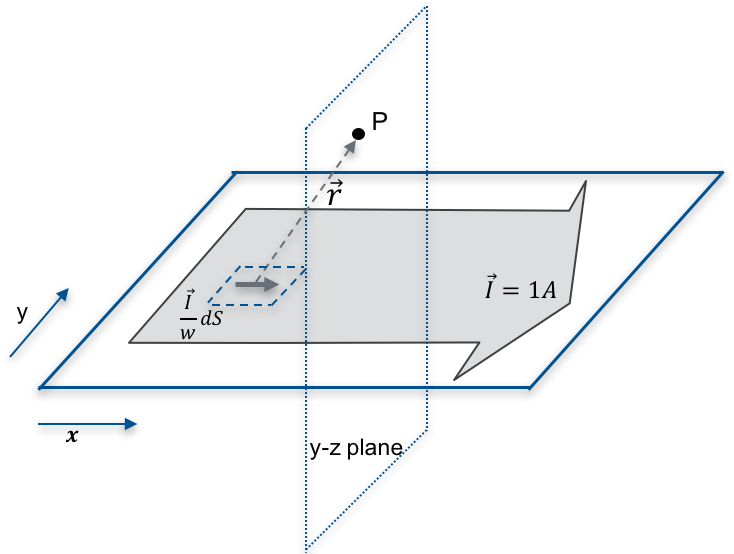
\includegraphics[scale=0.9]{images/TL_L(2).pdf}
\caption{The vector $\vec{ r } $ pointing from the surface element to the observation point.}
\label{fig:TL_L(2)}
\end{center}
\end{figure}

With formula (\ref{eq. TL_L}) the magnetic field at each point on y-z plane can be solved through either analytical solution or Matlab solution. The energy of inductor can be calculated by following equation:
\begin{equation}
  W=\frac{1}{2}LI^{2}=\frac{1}{2}\underset { \Omega  }{\int }{ B H  } d\Omega
 \end{equation} 
 where $\textbf{H}$ is the auxiliary magnetic field and has a relation $\textbf{B}=\mu \textbf{H}$.

 pictures and calculation....
 use the function quiver of Matlab to plot our vector plot.
\begin{figure}[htbp]
\begin{center}
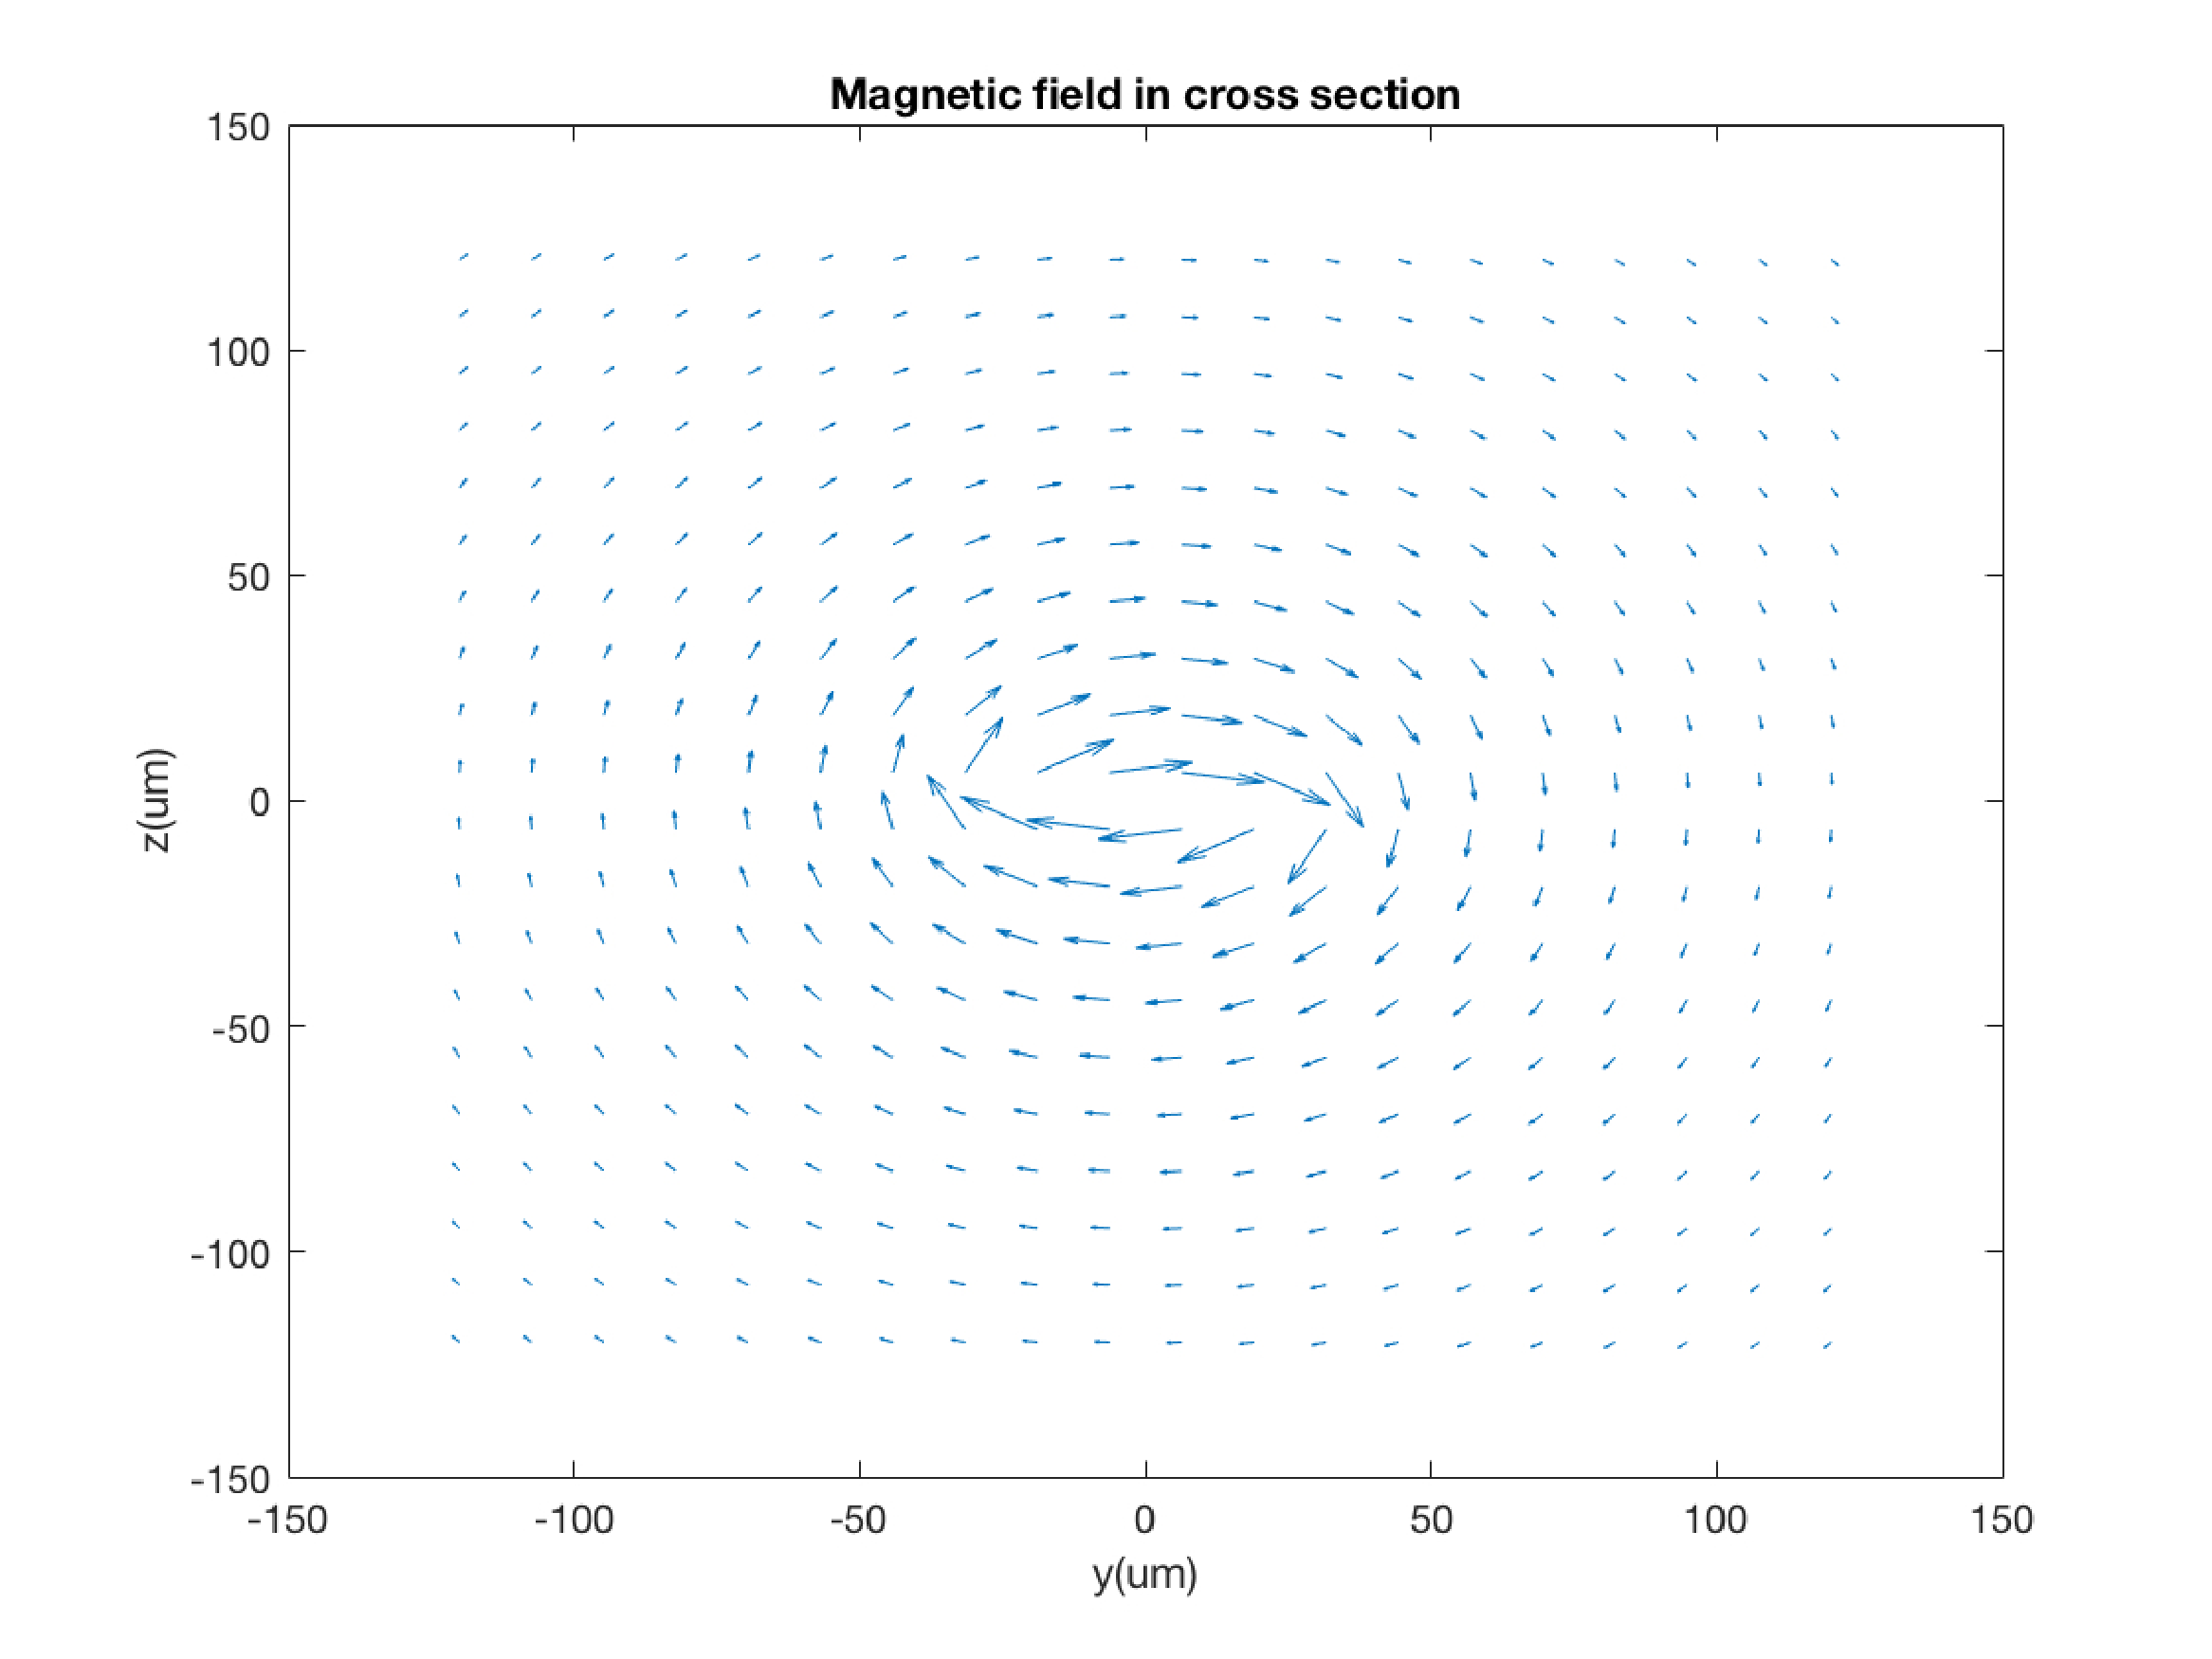
\includegraphics[scale=0.3]{images/TL_L.pdf}
\caption{Magnetic feld in cross section y-z plane.}
\label{fig:TL_L}
\end{center}
\end{figure}


\chapter{Numerical Treatment}
\section{Discretization}
Following Yee’s staggered grid approximation\cite{yee1966numerical}, voltage and current are discretized with separation of $\Delta x/2$ and $\Delta t/2$ in space and time respectively (See Figure \ref{fig:Discretisation}), which leads to a second-order accurate approximation. Voltage V(x,t) and current I(x,t) samples are then expressed as $ V\big(j\Delta x, (n+\frac{1}{2})\Delta t\big)$ and $ I\big((j+\frac{1}{2})\Delta x, n\Delta t\big)$, where j and n are integers. For reasons of simplicity, in the following text they will be replaced by $ V _{ j }^{ n+\frac{1}{2}}$ and ${ I }_{ j+\frac{1}{2} }^{ n }$. After discretization, the first-order derivative of voltage $\partial V(x,t)$ as well as current $\partial I(x,t)$ in space and time can be simply calculated with central difference method\cite{yang2012central}. 
% Discretisation figure
\begin{figure}[htbp]
\begin{center}
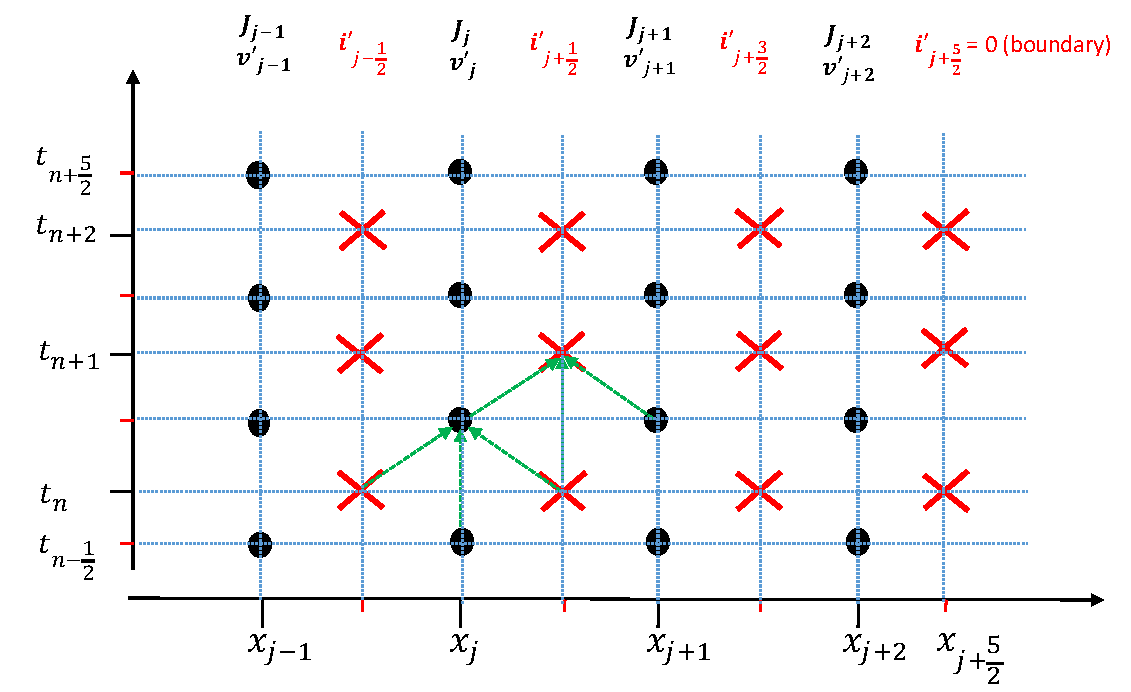
\includegraphics[scale=0.6]{images/Discretization}
\caption{Discretization along a staggered temporal and spatial grid.}
\label{fig:Discretisation}
\end{center}
\end{figure}

magic time step....

In order to solve these two partial differential equations, finite difference in time domain (FDTD) method is applied which owns second order accuracy.


Subsequently, the original Telegrapher's equations (\ref{eq:TLequation1}) and (\ref{eq:TLequation2}) are constructed as:
\begin{eqnarray}
\frac { { V }_{ j+1 }^{ n+\frac{1}{2} }-{ V }_{ j }^{ n+\frac{1}{2} } }{ \Delta x } & \approx & -L'\frac { { I }_{ j+\frac{1}{2} }^{ n+1 }-{ I }_{ j+\frac{1}{2} }^{ n } }{ \Delta t } -R' \widetilde{ i } _{ j+\frac{1}{2} }^{ n+\frac{1}{2} } \label{eq:TLequation3}\\
\frac{{ I }_{ j+\frac{1}{2} }^{ n } - { I }_{ j-\frac{1}{2} }^{ n }}{\Delta x} & \approx & -C'\frac {{ V }_{ j }^{ n+\frac{1}{2} }-{ V }_{ j }^{ n-\frac{1}{2} }}{ \Delta t }-w{J}_{j}^{n} \label{eq:TLequation4}
\end{eqnarray}
where, $ \widetilde{ i } _{ j+\frac{1}{2} }^{ n+\frac{1}{2} }$ is the ac (alternating current) component flowing between node j and node j+1 due to external RF source. w denotes width of simulated laser cavity. The ac component plays a major role especially in high frequency case, in which metal shows high resistance due to high frequency while in low frequency its resistance can be neglected. In active mode-locking with RF source, the modulation frequency is usually in order of $10^{10}$ Hz and metal resistance can reach several Ohms at such high frequency. Therefore, the influence of conductor resistance have to be taken into account to realize good agreement with real case. However, it is not suitable for use of traditional methods like Fourier Transformation (FT), which requires lots of samples in time domain. For this reason, it is not possible in this case to directly separate ac component of high frequency from the whole current during simulation.

Now that pure ac component cannot be simply obtained while resistance of transmission line at high frequency muss be taken into consideration, the problem was solved in another way by compromise. Instead of directly separating ac and dc component, temporal difference of ac component between adjacent time steps is considered to be feasible solution, which can be simply obtained by subtracting of Eqn. (\ref{eq:TLequation3}) at time ($n+\frac{1}{2}$) with that equation at previous time step ($n+\frac{1}{2}$), leading to:
\begin{equation}
\frac { { V }_{ j+1 }^{ n+\frac{3}{2} }-{ V }_{ j }^{ n+\frac{3}{2}}-({ V }_{ j+1 }^{ n+\frac{1}{2} }-{ V }_{ j }^{ n+\frac{1}{2} }) }{ \Delta x } \approx -L'\frac { { I }_{ j+\frac{1}{2} }^{ n+2 }-2{ I }_{ j+\frac{1}{2} }^{ n+1 }+{ I }_{ j+\frac{1}{2} }^{ n } }{ \Delta t } -R' (\widetilde{ i } _{ j+\frac{1}{2} }^{ n+\frac{3}{2} }-\widetilde{ i } _{ j+\frac{1}{2} }^{ n+\frac{1}{2} })\label{Eq:TL_substraction}
\end{equation}
The idea is, dc component as well as ac component with low frequency remains nearly unchanged after extremly short time step $\Delta t$ which is shorter than picosecond ($10^{-12}$ second) in the modeling. The variation of whole current at node $j+\frac{1}{2}$ is mainly due to variation of ac component with high frequency, which plays a key roll for increase of metal resistance. Hence, the variation of ac component can be approximately replaced with its corresponding variation of whole current. Besides, the current components have to be averaged in time for sake of consistence, the same with $J_{j}^{n}$, leading to:
\begin{equation}
\tilde{ i }_{ j+\frac { 1 }{ 2 }  }^{ n+\frac{3}{2} }-\tilde{ i }_{ j+\frac { 1 }{ 2 }  }^{ n+\frac{1}{2} }\approx{ I }_{ j+\frac { 1 }{ 2 }  }^{ n+\frac{3}{2} }-{ I }_{ j+\frac { 1 }{ 2 }  }^{ n+\frac{1}{2} } \approx \frac{{ I }_{ j+\frac { 1 }{ 2 }  }^{ n+2 }+{ I }_{ j+\frac { 1 }{ 2 }  }^{ n+1 }-({ I }_{ j+\frac { 1 }{ 2 }  }^{ n+1 }+{ I }_{ j+\frac { 1 }{ 2 }  }^{ n })}{2}\label{Eq:ac_Current}
\end{equation}
Then substituting the approximate treatment above to Eqn. (\ref{Eq:TL_substraction}),  a equation with only voltage and whole current can be obtained:
\begin{equation}
\frac { { V }_{ j+1 }^{ n+\frac{3}{2} }-{ V }_{ j }^{ n+\frac{3}{2}}-({ V }_{ j+1 }^{ n+\frac{1}{2} }-{ V }_{ j }^{ n+\frac{1}{2} }) }{ \Delta x } \approx -L'\frac { { I }_{ j+\frac{1}{2} }^{ n+2 }-2{ I }_{ j+\frac{1}{2} }^{ n+1 }+{ I }_{ j+\frac{1}{2} }^{ n } }{ \Delta t } -R' \frac{{ I }_{ j+\frac { 1 }{ 2 }  }^{ n+2 }-{ I }_{ j+\frac { 1 }{ 2 }  }^{ n }}{2}
\end{equation}

Finally, after rearrangement a recursive solution for Transmission line updating are explicitly expressed as:
\begin{eqnarray}
 \hspace{-8mm} { I }_{ j+\frac{1}{2} }^{ n+2 } &=& \frac { 4L' }{ 2L'+R'\Delta t }{ I }_{ j+\frac{1}{2} }^{ n+1 }-\frac { 2L'-R'\Delta t }{ 2L'+R'\Delta t }{ I }_{ j+\frac{1}{2} }^{ n }+\frac { { V }_{ j+1 }^{ n+\frac{3}{2} }-{ V }_{ j }^{ n+\frac{3}{2}}-{ V }_{ j+1 }^{ n+\frac{1}{2} }+{ V }_{ j }^{ n+\frac{1}{2} } }{  (\frac { L' }{ \Delta t } +\frac { R' }{ 2 })\Delta x }\label{eq:TL_I}\\
 \hspace{-8mm} { V }_{ j }^{ n+\frac{1}{2} } &=& { V }_{ j }^{ n-\frac{1}{2} } + \frac{ \Delta t }{ C'\Delta x } ({ I }_{ j-\frac{1}{2} }^{ n}-{ I }_{ j+\frac{1}{2} }^{ n } - w\Delta x\frac{{J}_{j}^{n+\frac{1}{2}}+{J}_{j}^{n-\frac{1}{2}}}{2}) \label{eq:TL_U}
\end{eqnarray}

\section{Modulation power}
Not only modulation frequency but also modulation power plays a key role in mode-locking. Even if QCL was modulated at near round trip frequency $f_{rt}$ , it can't be mode locked without enough modulation power. So it is essential to evaluate RF power for each simulation in order to analyze the modulation process. The RF source power can be easily calculated as modulation amplitude, signal function (since wave) as well as frequency are all known. But this power is total power and is larger than the power that was injected into QCL. Only the injected RF power will have influence on modulation.

The reflection coefficient $\Gamma$ is defined as:
\begin{equation}
\Gamma = \frac{Z_{QCL}-Z_{S}}{Z_{QCL}+Z_{S}}
\end{equation}

Two methods to estimate modulation power:

1. Through Fourier Transformation ac component can be easily separated at modulation frequency $f_{RF}$ from recorded whole current data over time. In the way, average RF voltage signal can also be obtained. Therefore, the injected RF-power to QCL is approximately:
\begin{equation}
 P_{RF}=\delta I* \delta V
 \end{equation}
where $\delta I$ and $ \delta V$ are current and voltage component at $f_{RF}$, respectively. 

2. Using the formula \cite{ramo2008fields}, which is used for calculation of small signal current modulation:
\begin{equation}
{ P }_{ diss }=\frac { \delta { I }_{ QCL }^{ 2 }*Re[{ Z }_{ QCL }] }{ 2 }
\end{equation}

where, $\delta { I }_{ QCL }$ is induced current variation due to RF source and ${ Z }_{ QCL }$ is the impedance of QCL at modulation frequency $Z_{QCL}=\sqrt{\frac{R'+j2\pi f_{RF}L'}{G'+j2\pi f_{RF}C'}}$. The distributed conductance G can be obtained through I-V characteristic curve of QCL.

--> rewrite this section 

\chapter{Simulation Results}
The laser simulated in this work is based on doped $GaAs/Al_{x}Ga_{1-x}As$, which is 3 mm-long, 60 $\mu m$ wide, with height of 10 $\mu m$ metal-metal QCL. It is driven at 77 K and has an emission frequency of 3.8 THz. The average doping level of the active region is $5\times 10^{16} cm^{3}$. Its well and barrier widths are 4.6/9.8/2.6/9.0/4.4/17.6 nm.

...QCL structure...

\begin{figure}[htbp]
\begin{center}
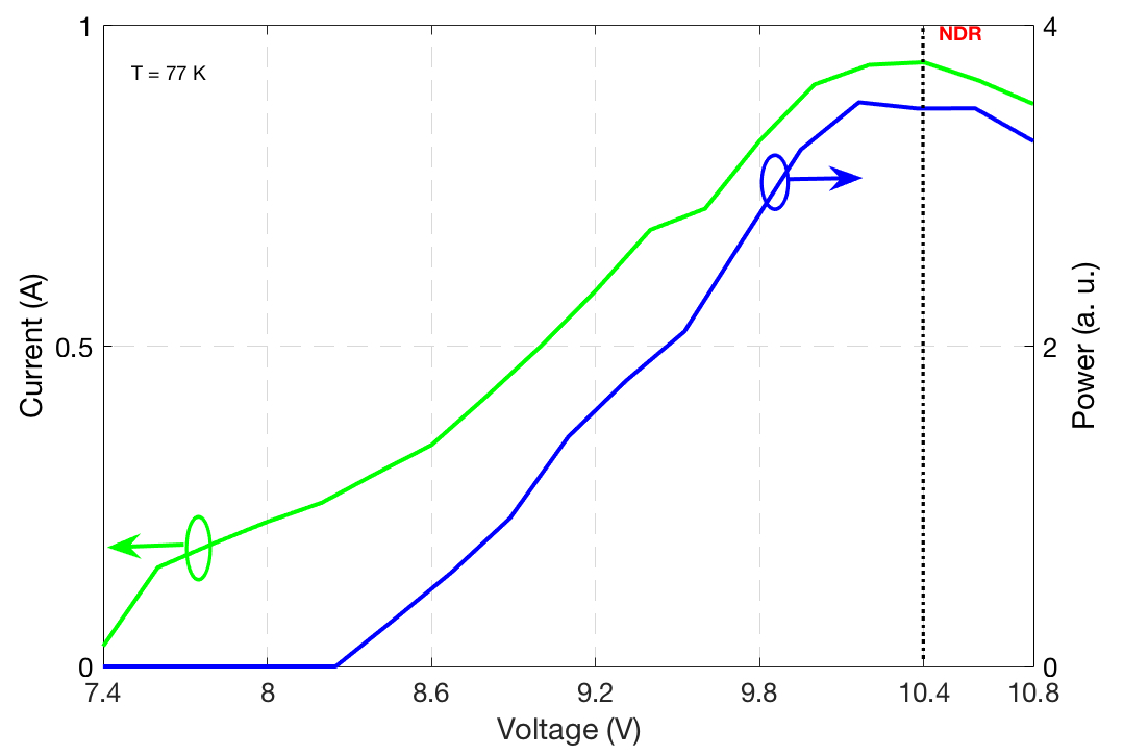
\includegraphics[scale=0.6]{images/IVCURVE.pdf}
\caption{voltage-current–power characteristics of simulated QCL.}
\label{fig:IVcurve}
\end{center}
\end{figure}

\begin{figure}[htbp]
\begin{center}
\includegraphics[scale=0.8]{images/withoutRF.eps}
\caption{Frequency spectrum of simulated QCL.}
\label{fig:withoutRF}
\end{center}
\end{figure}

Fig. \ref{fig:IVcurve} shows the voltage-current–power characteristics of the QCL, which was obtained by simulating the QCL under a series of bias from 7.4 V to 10.8 V. The QCL has a threshold voltage $V_{th}$ of 8.4 V, which means, under that there will be no lasing. Starting from $V_{th}$, the output power will increase exponentially with higher voltage until tunneling phenomena occurs. At this area, QCL owns negative differential resistance (NDR) which is similar as tunneling diode. A large amount of injected electrons due to increased input voltage will directly pass active region through tunneling rather than transition from upper and lower laser levels accompanied with emission of phonons. Therefore, they will not contribute to laser output power.

Description of I-V-P curve, e.g. threshold and kink, negative differential resistance (NDR)...............

In order to obtain a accuracy round trip frequency of this QCL, beatnote was used by Fourier transform of its output power. As Fig. \ref{fig:beatnote_noRF} shows,  beatnote of the simulated QCL without modulation, its round trip frequency $f_{rt}$ is around 13.34 GHz.
\begin{figure}[htbp]
\begin{center}
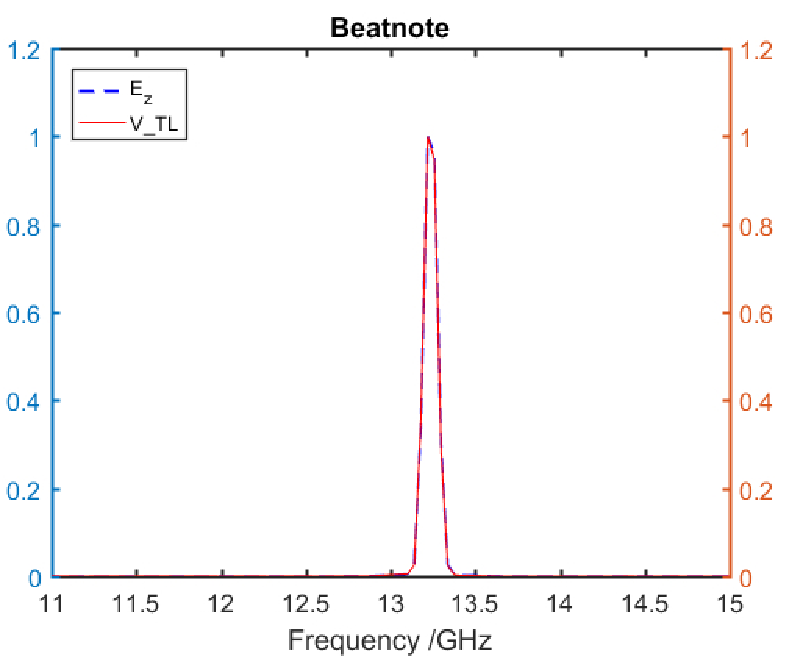
\includegraphics[scale=0.8]{images/beatnote_noRF.pdf}
\caption{Beatnote of the QCL without modulation.}
\label{fig:beatnote_noRF}
\end{center}
\end{figure}


\section{Simulation setup}
The source of simulated QCL consists of a DC voltage source and a RF source, which are combined through bias-T. 
% Power calculation of injected RF

replace this ugly picture with that from petar
\begin{figure}[htbp]
\begin{center}
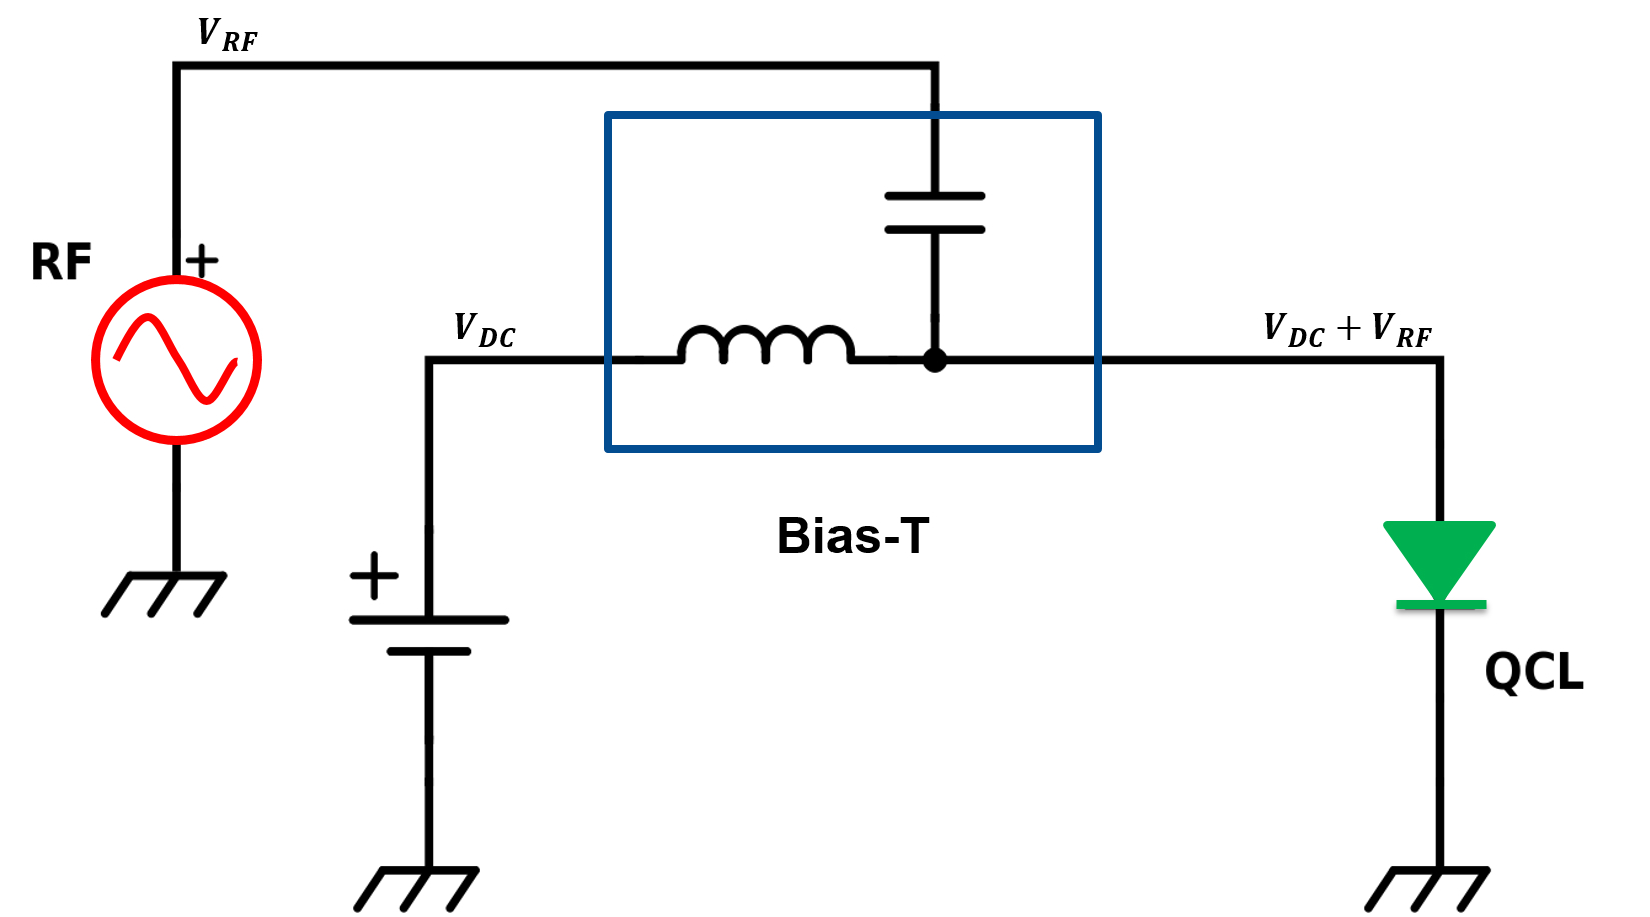
\includegraphics[scale=0.4]{images/schematicSETUP}
\caption{schematic scheme.}
\label{fig:schematicSETUP}
\end{center}
\end{figure}



\begin{table}[]
\centering
\caption{Simulation parameters}
\label{SIMparameter}
\begin{tabular}{llll}
\hline
\multicolumn{1}{|l|}{\textbf{Name}}  & \multicolumn{1}{l|}{\textbf{Symbol}} & \multicolumn{1}{l|}{\textbf{Value}} & \multicolumn{1}{l|}{\textbf{Unit}}         \\ \hline
\multicolumn{1}{|l|}{Cavity length}  & \multicolumn{1}{c|}{$L_{tot}$}       & \multicolumn{1}{c|}{3}              & \multicolumn{1}{c|}{mm}                    \\ %\hline
\multicolumn{1}{|l|}{Cavity width}  & \multicolumn{1}{c|}{$w$}   & \multicolumn{1}{c|}{60}              & \multicolumn{1}{c|}{um}                    \\ %\hline
\multicolumn{1}{|l|}{Doping density} & \multicolumn{1}{c|}{$D_{p}$ }        & \multicolumn{1}{c|}{1.5E16}         & \multicolumn{1}{c|}{$cm^{-3}$} 			   \\ %\hline
\multicolumn{1}{|l|}{Period length}  & \multicolumn{1}{c|}{$L_{p}$}         & \multicolumn{1}{c|}{54.8}           & \multicolumn{1}{c|}{nm}                    \\ %\hline
\multicolumn{1}{|l|}{Overlap factor} & \multicolumn{1}{c|}{$\Gamma$}          & \multicolumn{1}{c|}{0.8}          & \multicolumn{1}{c|}{}                      \\ 
 \multicolumn{1}{|l|}{Cavity loss}     &  \multicolumn{1}{c|}{$L_{\alpha}$}    &\multicolumn{1}{c|}{13}				&  \multicolumn{1}{c|}{$1/cm$} 						\\ \hline
\end{tabular}
\end{table}


\section{Results}
After 100 round trips simulation, a clear short pulse was observed, as Figure \ref{fig:FWHM} shows, from 4610 to 4690 ps in corresponding to 164 $T_{rt}$. Its Full Width at Half Maximum (FWHM) in this modeling is around 11.6 ps, which shows extremely good agreement with experiment result 11 ps\cite{gellie2010injection}.

\subsection{Modulation with different power} 
optimal power injection and comparison with lack of enough RF power as modulation
\subsection{Modulation with different frequency} 
"Pulling effect" and locking range

\begin{figure}[htbp]
\begin{center}
\includegraphics[scale=0.9]{images/FWHM.eps}
\caption{Singel pulse from simulation.}
\label{fig:FWHM}
\end{center}
\end{figure}

\section{Comparison with experiment}
Describe and argue this simulation results with experiment results from paper "Generating ultrafast pulses of light from qcls"
\chapter{Conclusion}



% -----------------------------
%   LITERATUR VERZEICHNIS
% -----------------------------

%\addcontentsline{toc}{chapter}{List of Figures}
%\listoffigures

\renewcommand*{\bibname}{Bibliography} % Using "Sources" as the title of the section
\bibliography{reference}{}
\addcontentsline{toc}{chapter}{Bibliography}

\bibliographystyle{ieeetr}

\end{document}
